% Generated by analysis_provenance/make_supp_sections.py. Do not edit.
\section{Closed forms against Monte Carlo: all six panels}\label{sup:theoryfig}
\begin{figure}[h]
\centering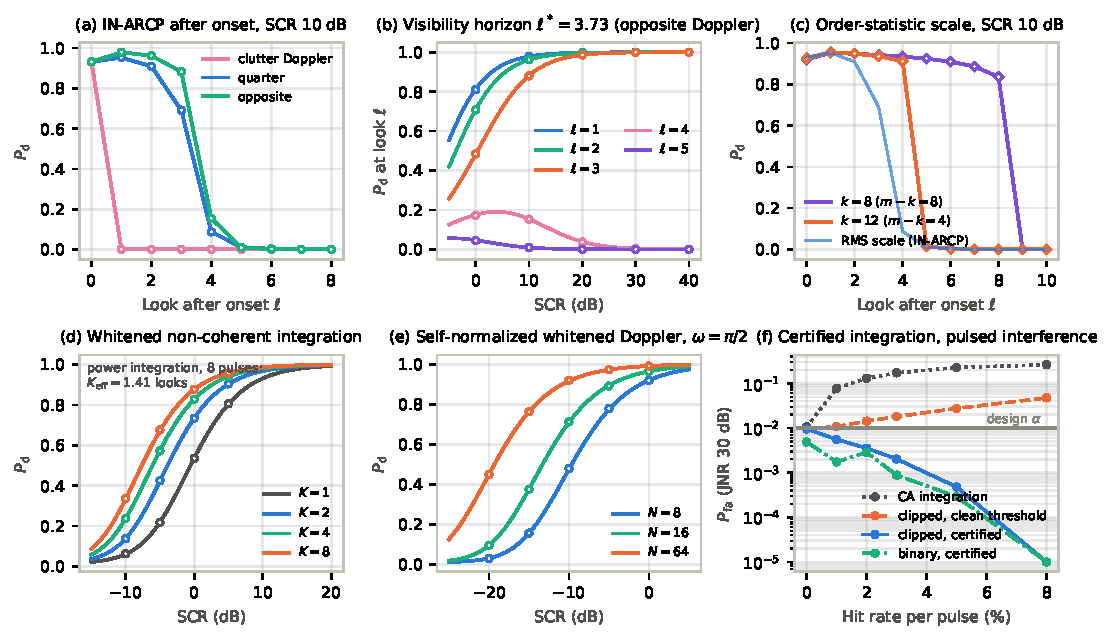
\includegraphics[width=.95\textwidth]{fig_theory_full.pdf}
\caption{Closed forms (lines) against Monte Carlo (markers; $10^5$ episodes per point in (a), (c) and (f), $5\times10^4$ in (b) and (d), $10^4$ to $2.5\times10^4$ in (e)) at the true coefficient, AR(1) compound-Gaussian clutter with $\rho=0.93e^{-0.2\mathrm j}$, lognormal texture, $m=16$, $P_{\rm fa}=0.01$. Panels (a)--(c) and (f) are those of Fig.~\ref{M-fig:theory} of the paper, where (f) appears as its panel (d) and (c) here adds the RMS-scale law for reference. The two panels shown only here are (d), the integration law \eqref{M-eq:dwellpd}, and (e), P-ANMF with unknown Doppler. JNR in (f): interference-to-clutter-plus-noise power ratio.}
\end{figure}

\section{Dwell detection on IPIX}\label{sup:dwell}
\begin{table}[h]
\centering\small
\caption{SCR (dB) for $P_{\rm d}=0.5$ and $0.9$ over an 8-pulse dwell: persistent Swerling-1 target with random Doppler from the first dwell pulse (IPIX, conformal thresholds). $\le-5$: reached at the lowest SCR tested; n.r.: not reached at 25~dB.}
\label{tab:dwellsup}
\begin{tabular}{lccc}
\toprule
 & \multicolumn{2}{c}{$\alpha=0.01$} & $0.001$\\
\cmidrule(lr){2-3}
 Detector & $P_{\rm d}=0.5$ & $0.9$ & $0.5$\\
\midrule
PAMF-H & $\le-5$ & 5.1 & -4.3\\
Integration, AR(4) & $\le-5$ & 7.0 & -1.6\\
Integration, AR(1) & -4.4 & 8.3 & -0.1\\
Clipped, OS scale & -2.3 & 13.0 & n.r.\\
Binary, OS scale & -1.2 & 14.5 & n.r.\\
ANMF-SCM & -0.2 & 20.3 & 9.5\\
ANMF-Tyler & 0.4 & 20.3 & 9.8\\
P-ANMF & 0.2 & n.r. & n.r.\\
IN-ARCP, first look & -1.2 & 11.0 & 1.9\\
Power OS, first look & 9.4 & 19.5 & 14.3\\
\bottomrule
\end{tabular}

\end{table}
